\documentclass[12pt]{article} % use larger type; default would be 10pt

\usepackage[utf8]{inputenc} % set input encoding (not needed with XeLaTeX)

\usepackage{graphicx}

\usepackage{listings}
\usepackage[scaled]{beramono}
\usepackage[T1]{fontenc}

\lstset{ basicstyle= \ttfamily, language=Logo, tabsize = 4, showspaces= false, showstringspaces=false}







%%% The "real" document content comes below...

\title{REALLY BIG IMPRESSIVE TITLE}
\author{Andrew Rosen \qquad Brendan Benshoof }
\date{} % Activate to display a given date or no date (if empty),
         % otherwise the current date is printed 

\begin{document}
\maketitle

\section{Problem Space}



\subsection{Chord}

The Chord protocol \cite{Chord} takes in some key and returns the identity (ID) of the node responsible for that key.  These keys are generated by hashing a value of the node, such as the IP address, or by hashing  the filename of a file.  The hashing process creates a $m$-bit hash identifier\footnote{In our simulation, this hash-id is randomly generated for each node.}, where $2^m$ is the maximum number of nodes in the network.

The nodes are then arranged in a ring from the lowest hash-value to highest.  Chord then takes the hashed files and places each in the node that has the same hashed identifier as it.  If no such node exists, the node with the first identifier that follows this value.  This node responsible for the key $\kappa$ is called the $successor$ of $\kappa$, or $successor(\kappa)$.  Since we are dealing with a circle, this assignment is done in module $2^m$ space.  For example, if there were some portion of the network with nodes 20, 25, and 27, node 25 could be responsible for the files with the keys [21,22,23,24,25]. If node 25 were to decide to leave the network, it would inform node 27, who would then be responsible for all the keys node 25 was covering. An example Chord network is drawn in in Figure \ref{chordreal}.

With this scheme, we can reliably find the node responsible for some key by asking the next node in the circle for the information, who would then pass the request through the circle until the successor was found.  We can then proceed to directly connect with the successor to retrieve the file.  This naive approach is largely inefficient, and is a simplification of the lookup process, but it is the basis of how Chord theoretically works.

To speed up the lookup time, each node stores not just its successor, but also the locations of up to $m$ other nodes in the network a \emph{finger table}.  The $i$th entry of node $n$'s \emph{finger table} will be the location of $successor(n+2^{i-1})$ $mod$ $2^m$\footnote{Because hash values won't be perfectly distributed, it is perfectly acceptable to have duplicate entries in the \emph{finger table}}. When a node $n$ is told to find some key, $n$ looks to see if the key is between $n$ and $successor(n)$ and return $successor(n)$'s information to the requester. If not, it looks for the entry in the finger table for the closest preceding node $n'$ it knows and asks $n'$ to find the successor.  This allows each step in the to skip up to half the nodes in the network, giving a $\log_2(n)$ lookup time.   The code for these processes used for the simulation are shown in ALGORITHM SOMETHING OR ANOTHER.


Because nodes can constantly join and leave the network, maintenance is essential to keeping the finger tables accurate.

Further details and the specifics of maintenance and protocol can be found in Stioca et al.'s paper on Chord \cite{Chord}.



\section{Goals of Modeling and Simulation}
We chose to specifically examine the formation period of a Chord Hash. The cited papers discuss how a single node can join a Chord Hash but gloss over the initial state for building a Chord Hash from scratch in a distributed setting. This made general simulation of Chord difficult as at least an initial chord ring had to be "boot-strapped" as a pre-connected initial ring so that other nodes can join it. Because this was an architecture level design problem, we were not interested in parts of the Chord Hash technique like the behavior of the actual network topology, latency, and server capacity. Thus we make a series of simplifying assumptions.

For this simulation we only consider the over-lay topology, not the underlaying topology of the network, thus we create links with the assumption that nodes have the potenital to link into a clique (and in many small network cases the system does actually form a clique).

It is important that our latency for this simulation be varied, but only so that behaviors that only occur in race condition could become apparent if they existed but for our purposes the exact qualities of that variance could be left vague. This allowed us to use travel from node to node in a 2D space


\section{Developed Models}




\begin{lstlisting}
to perform-task
	do-something
end
\end{lstlisting}


\section{Experiments}

\section{Results}

\section{Conclusion and Future Work}



\begin{figure}
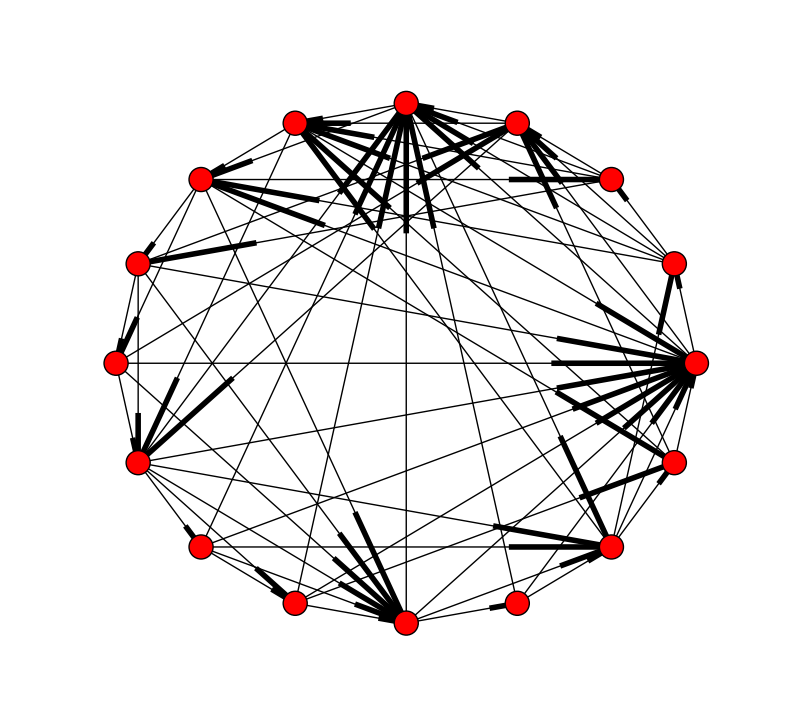
\includegraphics[width=\linewidth]{chordreal}
\caption{An example size 16 network produced by the simulation.  The lines edges are incoming edges.  Note that, unlike in an ideal Chord network, nodes have differing numbers of incoming and outgoing edges.}
\label{chordreal}
\end{figure}






\bibliographystyle{plain}
\bibliography{IRMLP}


\end{document}